% Results are provided in simulation_results.log
\begin{figure}
  \centering
  \begin{subfigure}{0.48\columnwidth}
    \centering
      \resizebox{\textwidth}{!}{%
      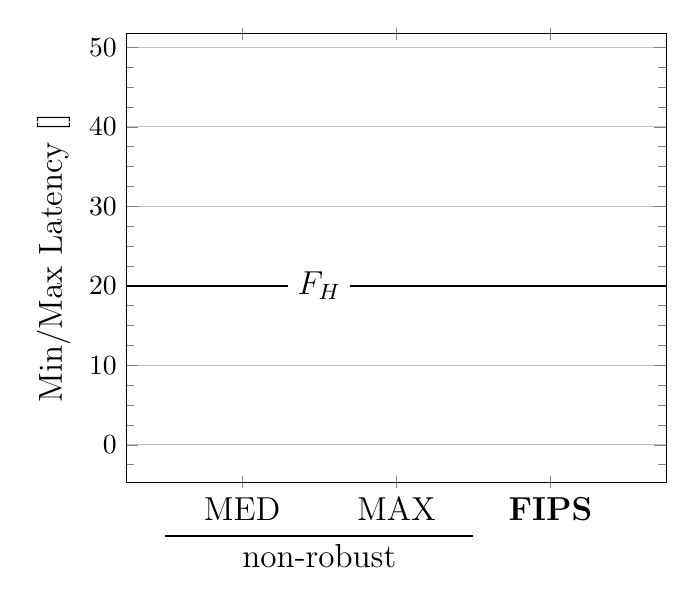
\begin{tikzpicture}
	\begin{axis}[
	      ylabel = {\large Min/Max Latency [\unit{\ms}]},
	      xtick = {1,2,3},
	      xtick align=center, 
	      minor y tick num = 3,
	      enlarge y limits,
	      xmin = 0.25, xmax = 3.75,
	      ymin = 0, ymax = 47,
	      ymajorgrids,
	      xticklabels = {\large MED, \large MAX, \large \textbf{FIPS}},
	      clip=false,
	    ]

	    \draw[thick] (axis cs:0.25,20) -- (axis cs:3.75,20);
	    \node[fill=white] at (axis cs: 1.5,20) {\large $\ete{F_H}$};

	    % CORE_AGV0_00
	    \intervalplt at (1, 4.983, 45.136);
	    \intervalplt at (2, 16.708, 24.55);
	    \intervalplt at (3, 17.918, 18.017);

	    \draw[thick] (axis cs: 0.5,-11.5) -- (axis cs: 2.5,-11.5);
	    \node at (axis cs: 1.5,-14) {\large non-robust};
	\end{axis}
      \end{tikzpicture}
      }
  \end{subfigure}
  \hfill
  \begin{subfigure}{0.48\columnwidth}
    \centering
      \resizebox{\textwidth}{!}{%
	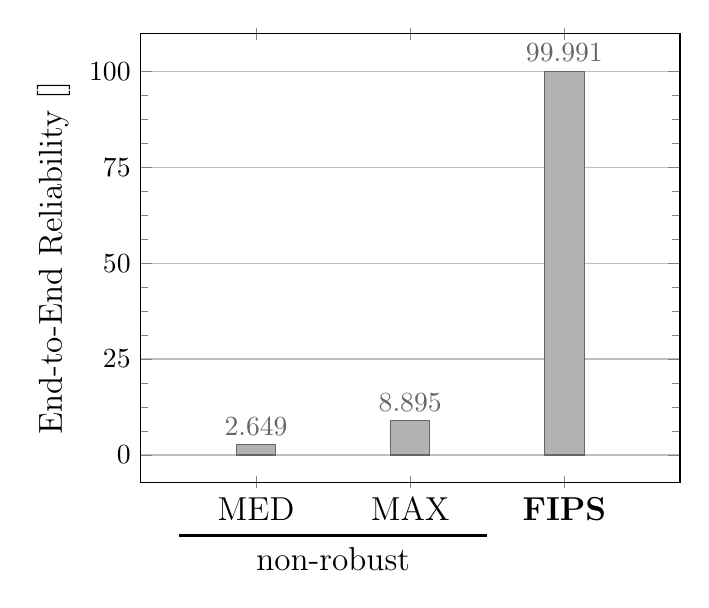
\begin{tikzpicture}
	  \begin{axis}[
		ybar,
		ylabel = {\large End-to-End Reliability [\unit{\percent}]},
		ytick = {0, 25, 50, 75, 100},
		xtick align=center, 
		minor y tick num = 3,
		ymajorgrids,
		enlarge y limits,
		xtick = {1,2,3},
		xmin = 0.25, xmax = 3.75,
		xticklabels = {\large MED, \large MAX, \large \textbf{FIPS}},
		nodes near coords,
		nodes near coords align={vertical},
		nodes near coords style={/pgf/number format/.cd,precision=3},
		clip=false,
	    ]

	      \addplot[black!60,fill=black!30,bar width=0.5cm] coordinates {(1, 2.6491) (2, 8.8948) (3, 99.9914)};

	      \draw[thick] (axis cs: 0.5,-21) -- (axis cs: 2.5,-21);
	      \node at (axis cs: 1.5,-27) {\large non-robust};
	  \end{axis}
	\end{tikzpicture}
      }
  \end{subfigure}
  \caption{Simulation results showing the achieved QoS of $F_H$.} \label{fig:simulation}
\end{figure}

